%-------------------------------------------------------------------------------
% This file provides a skeleton ATLAS note.
% \pdfinclusioncopyfonts=1
% This command may be needed in order to get \ell in PDF plots to appear. Found in
% https://tex.stackexchange.com/questions/322010/pdflatex-glyph-undefined-symbols-disappear-from-included-pdf
%-------------------------------------------------------------------------------
% Specify where ATLAS LaTeX style files can be found.
\newcommand*{\ATLASLATEXPATH}{latex/}
% Use this variant if the files are in a central location, e.g. $HOME/texmf.
% \newcommand*{\ATLASLATEXPATH}{}
%-------------------------------------------------------------------------------
\documentclass[NOTE, atlasdraft=true, texlive=2016, UKenglish]{\ATLASLATEXPATH atlasdoc}
% The language of the document must be set: usually UKenglish or USenglish.
% british and american also work!
% Commonly used options:
%  atlasdraft=true|false This document is an ATLAS draft.
%  texlive=YYYY          Specify TeX Live version (2016 is default).
%  coverpage             Create ATLAS draft cover page for collaboration circulation.
%                        See atlas-draft-cover.tex for a list of variables that should be defined.
%  cernpreprint          Create front page for a CERN preprint.
%                        See atlas-preprint-cover.tex for a list of variables that should be defined.
%  NOTE                  The document is an ATLAS note (draft).
%  PAPER                 The document is an ATLAS paper (draft).
%  CONF                  The document is a CONF note (draft).
%  PUB                   The document is a PUB note (draft).
%  BOOK                  The document is of book form, like an LOI or TDR (draft)
%  txfonts=true|false    Use txfonts rather than the default newtx
%  paper=a4|letter       Set paper size to A4 (default) or letter.

%-------------------------------------------------------------------------------
% Extra packages:
\usepackage{\ATLASLATEXPATH atlaspackage}
% Commonly used options:
%  biblatex=true|false   Use biblatex (default) or bibtex for the bibliography.
%  backend=bibtex        Use the bibtex backend rather than biber.
%  subfigure|subfig|subcaption  to use one of these packages for figures in figures.
%  minimal               Minimal set of packages.
%  default               Standard set of packages.
%  full                  Full set of packages.
%-------------------------------------------------------------------------------
% Style file with biblatex options for ATLAS documents.
\usepackage{\ATLASLATEXPATH atlasbiblatex}

% Package for creating list of authors and contributors to the analysis.
\usepackage{\ATLASLATEXPATH atlascontribute}

% Useful macros
\usepackage{\ATLASLATEXPATH atlasphysics}
\usepackage{xfrac}
% See doc/atlas_physics.pdf for a list of the defined symbols.
% Default options are:
%   true:  journal, misc, particle, unit, xref
%   false: BSM, heppparticle, hepprocess, hion, jetetmiss, math, process, other, texmf
% See the package for details on the options.

% Files with references for use with biblatex.
% Note that biber gives an error if it finds empty bib files.
\addbibresource{ANA-STDM-2020-17-INT1.bib}
\addbibresource{bib/ATLAS.bib}
\addbibresource{bib/CMS.bib}
\addbibresource{bib/ConfNotes.bib}
\addbibresource{bib/PubNotes.bib}

% Paths for figures - do not forget the / at the end of the directory name.
\graphicspath{{logos/}{figures/}}

% Add you own definitions here (file ANA-STDM-2020-17-INT1-defs.sty).
\usepackage{ANA-STDM-2020-17-INT1-defs}

%-------------------------------------------------------------------------------
% Generic document information
%-------------------------------------------------------------------------------

% Title, abstract and document
%-------------------------------------------------------------------------------
% This file contains the title, author and abstract.
% It also contains all relevant document numbers used for an ATLAS note.
%-------------------------------------------------------------------------------

% Title
\AtlasTitle{A simultaneous measurement of all charged particle properties in $Z$+jets events in $\sqrt{s}=13$ TeV $pp$ collisions using the ATLAS detector}

% Draft version:
% Should be 1.0 for the first circulation, and 2.0 for the second circulation.
% If given, adds draft version on front page, a 'DRAFT' box on top of each other page, 
% and line numbers.
% Comment or remove in final version.
\AtlasVersion{0.2}

%https://atlas-glance.cern.ch/atlas/analysis/analyses/details.php?id=5225

% Abstract - % directly after { is important for correct indentation
\AtlasAbstract{%
This support note describes a measurement of all charged particle properties in $Z$+jets events using the full Run 2 $pp$ collision dataset recorded by the ATLAS detector.  In particular, this is the first analysis to unfold data without binning and using a variable-length and high-dimensional phase space.  The phase space space is defined by the kinematic properties of all charged particles in boosted $Z\to\mu\mu$ events within a fiducial volume. The unfolding is implemented using the recently proposed OmniFold technique, which uses iteratively trained neural networks.  The analysis itself is broken into two part and this note serves as the reference for both parts.  The first part considers the case of a fixed number of observables (MultiFold) while the second part considers the case of all charged particles (OmniFold).
}

% Author - this does not work with revtex (add it after \begin{document})
%\author{The ATLAS Collaboration}

% Authors and list of contributors to the analysis
% \AtlasAuthorContributor also adds the name to the author list
% Include package latex/atlascontribute to use this
% Use authblk package if there are multiple authors, which is included by latex/atlascontribute
 \usepackage{authblk}
% Use the following 3 lines to have all institutes on one line
% \makeatletter
% \renewcommand\AB@affilsepx{, \protect\Affilfont}
% \makeatother
% \renewcommand\Authands{, } % avoid ``. and'' for last author
% \renewcommand\Affilfont{\itshape\small} % affiliation formatting
\AtlasAuthorContributor{Dag Gillberg}{a}{Ntuple production, analysis strategy, MC setup, advising Sandeep and Laura.}
\AtlasAuthorContributor{Sandeep Kaur}{a}{Data stability, jet composition studies, theory systematics.}
\AtlasAuthorContributor{Matt LeBlanc}{b}{Alternative observables.}
\AtlasAuthorContributor{Eric Metodiev}{e}{Short Term Associate.  Initial studies on dataset size.}
\AtlasAuthorContributor{Laura Miller}{a}{Ntuple production, MC setup, analysis strategy, event selection, data-MC comparison, systematics, statisitcal uncertaintiy using boot strapping.}
\AtlasAuthorContributor{Benjamin Nachman}{c}{Unfolding mechanics, event selection cross-check, analysis strategy, advising Adi.}
\AtlasAuthorContributor{Jennifer Roloff}{d}{Track jet studies.}
\AtlasAuthorContributor{Adi Suresh}{c,f}{Unfolding setup, stress-tests, and results.}
% \AtlasAuthorContributor{Second AtlasAuthorContributor}{b}{Author's contribution.}
% \AtlasAuthorContributor{Third AtlasAuthorContributor}{a}{Author's contribution.}
% \AtlasContributor{Fourth AtlasContributor}{Contribution to the analysis.}
% \author[a]{First Author}
% \author[a]{Second Author}
% \author[b]{Third Author}
\affil[c]{Lawrence Berkeley National Laboratory (LBNL)}
\affil[f]{University of California, Berkeley}
\affil[a]{Carleton University}
\affil[b]{European Center for Nuclear Research (CERN)}
\affil[d]{Brookhaven National Laboratory (BNL)}
\affil[e]{Massachusetts Institute of Technology (MIT)}
% \affil[b]{Another Institution}


% If a special author list should be indicated via a link use the following code:
% Include the two lines below if you do not use atlasstyle:
% \usepackage[marginal,hang]{footmisc}
% \setlength{\footnotemargin}{0.5em}
% Use the following lines in all cases:
% \usepackage{authblk}
% \author{The ATLAS Collaboration%
% \thanks{The full author list can be found at:\newline
%   \url{https://atlas.web.cern.ch/Atlas/PUBNOTES/ATL-PHYS-PUB-2016-007/authorlist.pdf}}
% }

% ATLAS reference code, to help ATLAS members to locate the paper
\AtlasRefCode{ANA-STDM-2020-17}

% ATLAS note number. Can be an COM, INT, PUB or CONF note
\AtlasNote{ANA-STDM-2020-17-INT1}

% Author and title for the PDF file
\hypersetup{pdftitle={ATLAS document},pdfauthor={The ATLAS Collaboration}}

%-------------------------------------------------------------------------------
% Content
%-------------------------------------------------------------------------------
\begin{document}

\maketitle

\tableofcontents

% List of contributors - print here or after the Bibliography.
%\PrintAtlasContribute{0.30}
%\clearpage

\clearpage

\section{Executive Summary}
\label{sec:exec}

\subsection{Target}

This analysis uses an innovative machine learning method~\cite{1911.09107} to perform an unbinned, variable- and high-dimensional unfolding using $Z$+jets events. As the first search using these new techniques, we limit the phase space to relatively high $p_T$ $Z$ bosons in the $Z\rightarrow\mu\mu$ channel.   The analysis uses the full Run 2 dataset and targets summer/fall 2021.

\subsection{Context}

While there is no other measurement that is unbinned, variable- and high-dimensional, there are a variety of related binned measurements of specific observables.   These include track-based observables in inclusive $Z$+jets events at $\sqrt{s}=8$ TeV~\cite{STDM-2015-14} and various measurements of hadronic final states using tracks~\cite{STDM-2018-57,STDM-2017-33,STDM-2017-16}.  None of these measurements are directly comparable to the one presented in this analysis because of the topology and/or the phase space.  However, as we are using a new methodology for the first time, one of the goals of this paper is to compare the method with standard techniques (e.g. Iterative Bayesian Unfolding~\cite{DAGOSTINI1995487,1974AJ.....79..745L,Richardson:72}) in addition to presenting the new unbinned data.

\subsection{Contributors}

\PrintAtlasContribute{0.30}

\clearpage

\section{Change Log}

\begin{itemize}
\item Version 0.1: Initial version, to be used for the editorial board request.
\end{itemize}

\clearpage

%-------------------------------------------------------------------------------
\section{Introduction}
\label{sec:intro}
%-------------------------------------------------------------------------------

The goal of the Large Hadron Collider (LHC) is to infer properties of nature at subnuclear length scales.   One strategy for data analysis is to use models like the Standard Model (SM) and its extensions to fit parameter values to data.  This is an effective strategy that has been used to measure Standard Model couplings and masses as well as to constrain the strength of new physics extensions of the SM.  A key limitation of this parametric approach is that the final result cannot be easily used to infer properties of other parameters or reinterpreted in the context of a different model.  An alternative strategy is to correct data for detector effects in order to measure differential cross sections.  These \textit{unfolded} spectra can be reused for a variety of model interpretations.   Unfolding facilitates data preservation for reuse over time and comparisons across experiments.

The most widely used unfolding methods use various forms of regularized matrix inversion~\cite{DAGOSTINI1995487,Hocker:1995kb,Schmitt:2012kp}.  There are four challenges with these approaches that limit their usefulness.   First, the target observables must be specified prior to unfolding and cannot be changed after the measurement.  Similarly, the binning of the observables must be fixed at the start of the measurement.  Due to the binned nature of existing techniques, most measurements are limited to a small number of observables (usually one) to be simultaneously unfolded.  Finally, the existing methods are not able to account for auxiliary features that determine the resolution of the target observables and thus limit the precision of the measurement.

A variety of alternative unfolding method have been proposed to solve a subset of these challenges.   For example, some proposals avoid binning~\cite{Glazov:2017vni,Datta:2018mwd,Lindemann:1995ut,Aslan:2003vu} and others use machine learning to improve various aspects of the measurement precision~\cite{Gagunashvili:2010zw,Glazov:2017vni,Datta:2018mwd}.  Recently, three techniques have been proposed that have the potential to address all of the above challenges: OmniFold~\cite{1911.09107}, Conditional GAN Unfolding (CGU)~\cite{Bellagente:2019uyp}, and Conditional Normalizing Flow Unfolding (CNFU)~\cite{Bellagente:2020piv}.   The OmniFold approach scaffolds a simulation with a neural network to perform high- and variable-dimensional reweighting.  The CGU and CNFU methods use neural networks to generate corrected events given detector-level events.  

This analysis uses the OmniFold approach to perform the first high- and variable-dimensional unbinned measurement.  In contrast to the CFU and CNFU methods, OmniFold can naturally account for point-cloud nature of collider events.  Furthermore, OmniFold reduces to the widely studied Iterative Bayesian Unfolding approach~\cite{DAGOSTINI1995487} when the inputs are binned.  Finally, by using reweighting instead of direct generative modeling, the neural networks need to only learn small corrections to the simulation instead of learning the full probability density of the data.   The physical system chosen for the measurement is the hadronic activity in boosted $Z$ boson events.  Leptonically decaying $Z$ bosons can be identified with high purity and efficiency.  The rest of the event can then be studied with little bias from the event selection.  Charged particles are used due to the precision with which they can be measured.  These events have many tens of charged particles each with a momentum and electric charge and thus the target phase space is about 100-dimensional.

This note is organized as follows.  First, Sec.~\ref{sec:samples} introduces the data and simulated event samples used for the analysis.  Then, Sec.~\ref{sec:objects} describes the objects used in the analysis (in particular, charged particles and tracks).  The analysis methodology is disucssed in Sec.~\ref{sec:strategy} and the prescription for systematic uncertainties appears in Sec.~\ref{sec:uncerts}.  Results are presented in Sec.~\ref{sec:result} and the note concludes in Sec.~\ref{sec:conclusion}.

%-------------------------------------------------------------------------------
\section{Event samples}
\label{sec:samples}
\input{4_data_MC}

%-------------------------------------------------------------------------------
\section{Objects}
\label{sec:objects}
\subsection{Event selection}
\label{sec:selection}

Initial event selection is outlined in table~\ref{lab:eventsel}. This is primarily designed to remove problematic and background events in favour of the $Z\rightarrow\mu\mu + \text{jets}$ signal process. The various cuts are discussed in more detail below.

\begin{table}[h!]
    \centering
    \begin{tabular}{l|l}
         \hline
    \textbf{Event Selection} & \textbf{Description} \\ \hline
    Good Runs List & Event must be part of GRL \\ \hline
    Event Cleaning & No LAr, tile calorimeter, or tracker errors. Event is complete. \\ \hline
    Trigger & Single muon trigger: \\
    & \texttt{HLT\_mu20\_iloose\_L1MU15\_OR\_HLT\_mu50} (2015) \\
    & \texttt{HLT\_mu26\_ivarmedium\_OR\_HLT\_mu50} (2016-18) \\ \hline
    Primary Vertex & $N_{PV}\geq1$ \\ \hline
    Muons & $N_{\text{muons}}\geq2$ \\
          & Opposite charges \\
          & Pass TTVA recommendations for muons \\
          & $81\leq m_{\ell\ell} (\text{GeV})\leq 101$ \\
          & $p_{\text{T},\ell\ell}\geq200$ GeV \\ \hline
    \end{tabular}
    \caption{Overview of the applied event selection.}
    \label{lab:eventsel}
\end{table}

\subsubsection{Event Requirements}
The first requirement is that the event must be a part of the ATLAS Good Run Lists (GRL). These are discussed in section~\ref{sec:samples}.

Secondly, the events must pass event cleaning\footnote{The event cleaning procedure is outlined in \url{twiki: https://twiki.cern.ch/twiki/bin/view/Atlas/DataPreparationCheckListForPhysicsAnalysis}}. This removes events that:
\begin{itemize}
    \item Contain errors in the data collected in the LAr calorimeters (check for error on \texttt{xAOD::EventInfo::LAr})
    \item Contain errors in the data collected in the tile calorimeters (check for error on \texttt{xAOD::EventInfo::Tile})
    \item Contain errors in the silicon tracker data (check for error on \texttt{xAOD::EventInfo::SCT})
    \item Are incomplete due to a restart of the trigger, timing and control system (check for event flag in \texttt{xAOD::EventInfo::Core})
    \item Fail the Loose event cleaning requirement (\texttt{DFCommonJets\_eventClean\_LooseBad}). This is also applied to MC samples.
\end{itemize}

Additionally, it is required that the event in question have at least one primary vertex.

\subsubsection{Trigger Requirements}
\label{subsubsec:trigger}
Events are required to pass an unprescaled single muon trigger\footnote{The muon trigger recommendations can be found here: \url{twiki: https://twiki.cern.ch/twiki/bin/view/Atlas/MuonTriggerPhysicsRecommendationsRel212017}}, as outlined in table~\ref{lab:eventsel}.
The recommended trigger is dependent on the year in which the data was taken (or the year of the corresponding Monte Carlo sample).

\subsubsection{Di-Muon System Requirements}
The event is required to have at least two muons of opposite charge, with a dilepton mass between 81 GeV and 101 GeV in order to ensure the muons originate from a $Z$ boson.

Additionally, the muons must pass track-to-vertex association recommendations\footnote{Recommendations are given by the tracking group and are outlined here: \url{twiki: https://twiki.cern.ch/twiki/bin/view/AtlasProtected/TrackingCPEOYE2015}} as follows:

\begin{itemize}
    \item $|d_0^{BL}\text{significance}| < $ 3
    \item $|\Delta z_0^{BL}\sin\theta| < 0.5 $mm
\end{itemize}

where $d_0$ and $z_0$ represent the point along the track that is the closest approach to the beamspot.

The large $p_{\text{T},\ell\ell}$ cut of 200~GeV has been chosen to ensure that the balancing jet(s) have a high quantity of charged particles, as these are the primary subject of the analysis.
Events with a $p_{\text{T},\ell\ell}$ larger than 165~GeV are saved in order to study migration effects between truth and reconstructed events (i.e. events where the reconstructed $p_{\text{T},\ell\ell}$
is smaller than 200 GeV, but is larger than 200 GeV at truth level and vice versa).

\subsection{Detector-level objects}

\paragraph{Muons} are reconstructed using a combination of information from the muon spectrometer (MS) and the inner detector (ID). Occasionally, the ATLAS calorimeters are used to provide additional information for reconstruction. The reconstruction process is described in detail in reference~\cite{Aad:2016jkr}.
The muons are required to pass Medium quality selection using the \texttt{MuonSelectionTool}\footnote{The twiki detailing the MuonSelectionTool: \url{twiki: https://twiki.cern.ch/twiki/bin/view/Atlas/MuonSelectionToolR21}} and the \texttt{PflowLoose\_VarRad} isolation working point as given by
the \texttt{IsolationTool}\footnote{Information on the isolations WPs and the tool: \url{twiki: https://twiki.cern.ch/twiki/bin/view/AtlasProtected/RecommendedIsolationWPs}}. The simulated muons are also calibrated in order to correct for $p_\text{T}$ discrepancies between data and simulation~\cite{Aad:2016jkr}.
Kinematically, muons are required to have a minimum $\pt$ of 25~GeV, and have $|\eta|<2.4$.

\paragraph{Tracks} are reconstructed from charged-particle hits within the silicon- and straw-tube based inner tracking detectors. They are required to pass the Loose quality working point and to be associated with the primary vertex of the event using the Tight track-to-vertex association\footnote{Information on both the selection tool and the TTVA tool may be found here: \url{twiki: https://twiki.cern.ch/twiki/bin/view/AtlasProtected/TrackingCPRecsRun2Final}}.
The primary vertex is defined as the reconstructed vertex with the highest sum of associated track $\pt^2$. Tracks are required to have a $\pt>500$~\MeV~to be included in this measurement.  The track $\eta$ and $\phi$ coordinates come from the five-parameter track fit to $(\eta,\phi,q/p,d_0,z_0)$, and thus correspond to the track coordinates at the origin.
In addition, tracks which are associated with the muons are not considered part of the final track collection.

\paragraph{Jets} are reconstructed using the anti-$k_t$ algorithm~\cite{Cacciari:2008gp} with a radius parameter of $R=0.4$. Particle flow objects~\cite{Aaboud:2017aca} are used as input. The jets are calibrated using the recommended procedure for small-$R$ jets, this includes: MCJES calibration, global sequential calibration, and in-situ calibration.
Jets are required to have a calibrated $p_\text{T} > 10~\text{GeV}$ and rapidity $|y| < 4.4$\footnote{General recommendations are found here: \url{twiki: https://twiki.cern.ch/twiki/bin/view/AtlasProtected/JetEtmissRecommendationsR21}}. Note that while these are saved as objects during the analysis, they are not currently being used.

\paragraph{Track Jets} are also reconstructed using the anti-$k_t$ algorithm with a radius parameter of $R=0.4$. All tracks which pass the selection described above are used as input, and clustering is completed using \textsc{FastJet}~\cite{Cacciari:2011ma}.

\subsubsection{Overlap Removal}

There is a possibility that an electron may be misidentified as a jet during reconstruction, so in cases where the jet is found to be within $\Delta R < 0.2$ of a reconstructed electron, the jet is removed.
Additionally, a specialized overlap removal procedure must be applied between muons and jets due to a bug in the particle flow algorithm which results in secondary muon tracks being included in the particle flow objects.
The muon is preferentially kept in this case, so it does not limit our analysis as the jets are not currently used.

A summary of the detector level event selection can be found in table~\ref{tab:ObjCuts}.


\begin{table}[h!]
    \centering
    \begin{tabular}{l|l}
    \hline
     \textbf{Object} & \textbf{Additional Selection Criteria} \\ \hline
     Muons & $\pt>25~\GeV$, $|\eta|<2.4$ \\
           & Medium quality, pass isolation \texttt{PflowLoose\_VarRad} \\ \hline
     Jets (\texttt{AntiKt4EMPFlowJets}) & $\pt>10~\GeV$, $|y|<4.4$ \\
                                        & $\Delta R_{e,jet} > 0.2$ \\
                                        & Muon-PFlow jet overlap removal \\ \hline
     Tracks & $p_{\text{T}} > 500$ MeV \\
            & Loose Quality \\
            & Tight TTVA \\
            & Do not originate from a muon \\ \hline
     Track Jets & Input tracks must pass the above cuts \\ \hline
    \end{tabular}
    \caption{Object level cuts}
    \label{tab:ObjCuts}
\end{table}

\subsection{Particle-level objects}

Stable charged particles ($c\tau$ > 10 mm) are used to define the analog of tracks at particle-level. Charged-particles are required to have $\pt > 500$~\MeV~and $|\eta|<2.5$.
Muons are dressed using all photons within a radius of $R=0.1$ and identical kinematic cuts are applied to those used at the detector-level.
\texttt{TruthWZJets} are utilized at the particle-level, which are constructed utilizing the anti-$k_t$ algorithm with $R=0.4$ from all particle 4-vectors except for prompt leptons from $W$, $Z$, Higgs, and $\tau$ decay, and photons within a cone of $R=0.1$ around the prompt lepton.
Track jets at the particle-level are constructed using the same process as at the detector-level, but the charged particles are used as input.
Objects at particle-level, as well as the truth phase space, are summarized in table~\ref{tab:PLObjCuts}.

\begin{table}[h!]
    \centering
    \begin{tabular}{l|l}
    \hline
    \textbf{Object} & \textbf{Acceptance} \\ \hline
    Dressed Muons & $p_\text{T} > 25$ GeV, $|\eta| < 2.4$ \\\hline
    Jets (\texttt{TruthWZJets}) & $p_\text{T} > 10$ GeV, $|y|<4.4$ \\\hline
    Charged Hadrons & $p_\text{T}>500$ MeV, $|\eta|<2.5$  \\ \hline
    Track Jets & Charged hadrons used as input must pass above criteria \\ \hline
    Phase Space & At least two oppositely charged muons \\
    & $81<m_{\ell\ell}~\GeV<101$ \\
    & $p_{\text{T},\ell\ell}>200$ GeV \\ \hline
    \end{tabular}
    \caption{Fiducial object cuts and the truth phase space}
    \label{tab:PLObjCuts}
\end{table}

\subsection{Corrections to Monte Carlo samples}
\label{subsec:MCCorr}
\subsubsection{Pileup reweighting}
When events in MC samples are produced, the average interactions per bunch crossing, $\mu$, is assigned a certain value. This can differ from the values that are actually seen in the corresponding data, thus it is
necessary to correct the MC events such that the distribution of $\mu$ is equivalent to what is observed in data.

The \texttt{PileupReweightingTool}\footnote{Details can be found here: \url{twiki: https://twiki.cern.ch/twiki/bin/view/AtlasProtected/ExtendedPileupReweighting}} uses the $\mu$ and the run number assigned to the MC event along with the luminosity of the corresponding data in the same run number to determine the pileup weight to be applied to the event.
This requires that both the average $\mu$ distribution for the specific MC sample is available to the tool, as well as the files used to calculate the luminosity for the data. As we use unprescaled triggers in this analysis, the centrally produced lumicalc files corresponding to the GoodRunsLists in section~\ref{subsec:data} are used.
Configuration files for the tool for each MC sample are also provided centrally.
The pileup weight is then multiplied with the MC event weight in order to correct the $\mu$.

The tool also provides a scaling correction for data. The MC simulation for a given $\mu$ value is known to be too hard, therefore the average $\mu$ values in data are scaled down to account for this.

\subsubsection{Trigger scale factor}
There are differing trigger efficiencies between data and MC simulation, thus a correction in the form of a scale factor applied to the event weight is necessary for MC events. The triggers used in this analysis are outlined in section~\ref{subsubsec:trigger}.

\subsubsection{Muon scale factors}
Muon scale factors related to reconstruction efficiency, isolation efficiency, and track-to-vertex (TTVA) efficiency are derived from $J/\psi$ and $Z$ events using the tag-and-probe method for muons in the central region. The resulting scale factors are applied to the event weight in the same way as the trigger scale
factor\footnote{Addtional information on both the trigger and muon scale factors may be found in the muon analysis twiki: \url{twiki: https://twiki.cern.ch/twiki/bin/view/AtlasProtected/MCPAnalysisGuidelinesMC16}}.

\subsection{Data stability tests}
To check stability of data used for this analysis, rate for each year is calculated by dividing events to their corresponding luminosities. Luminosity per run is combined until summed up luminosities become either 2 fb$^{-1}$ or greater than this. Figure~\ref{fig:DataStability} depicts rate for year 2015 to 2018, where each time-ordered data bin contains 2 fb$^{-1}$ luminosity. The first bin shows rate for year 2015, bins 2--16 are for year 2016, bins 17--37 and 38--64 represent rate for year 2017 and 2018 respectively. Further, to consider those residual runs having combined luminosities smaller than 2 fb$^{-1}$, the last bin for each year is merged with the previous bin. The calculated average rate for year 2015--2018 is 2845 $\pm$ 4 and shows consistentency for each year. Figure~\ref{fig:DataStability} shows the stability of data for each year used in this analysis.
\begin{figure}[h!]
\centering
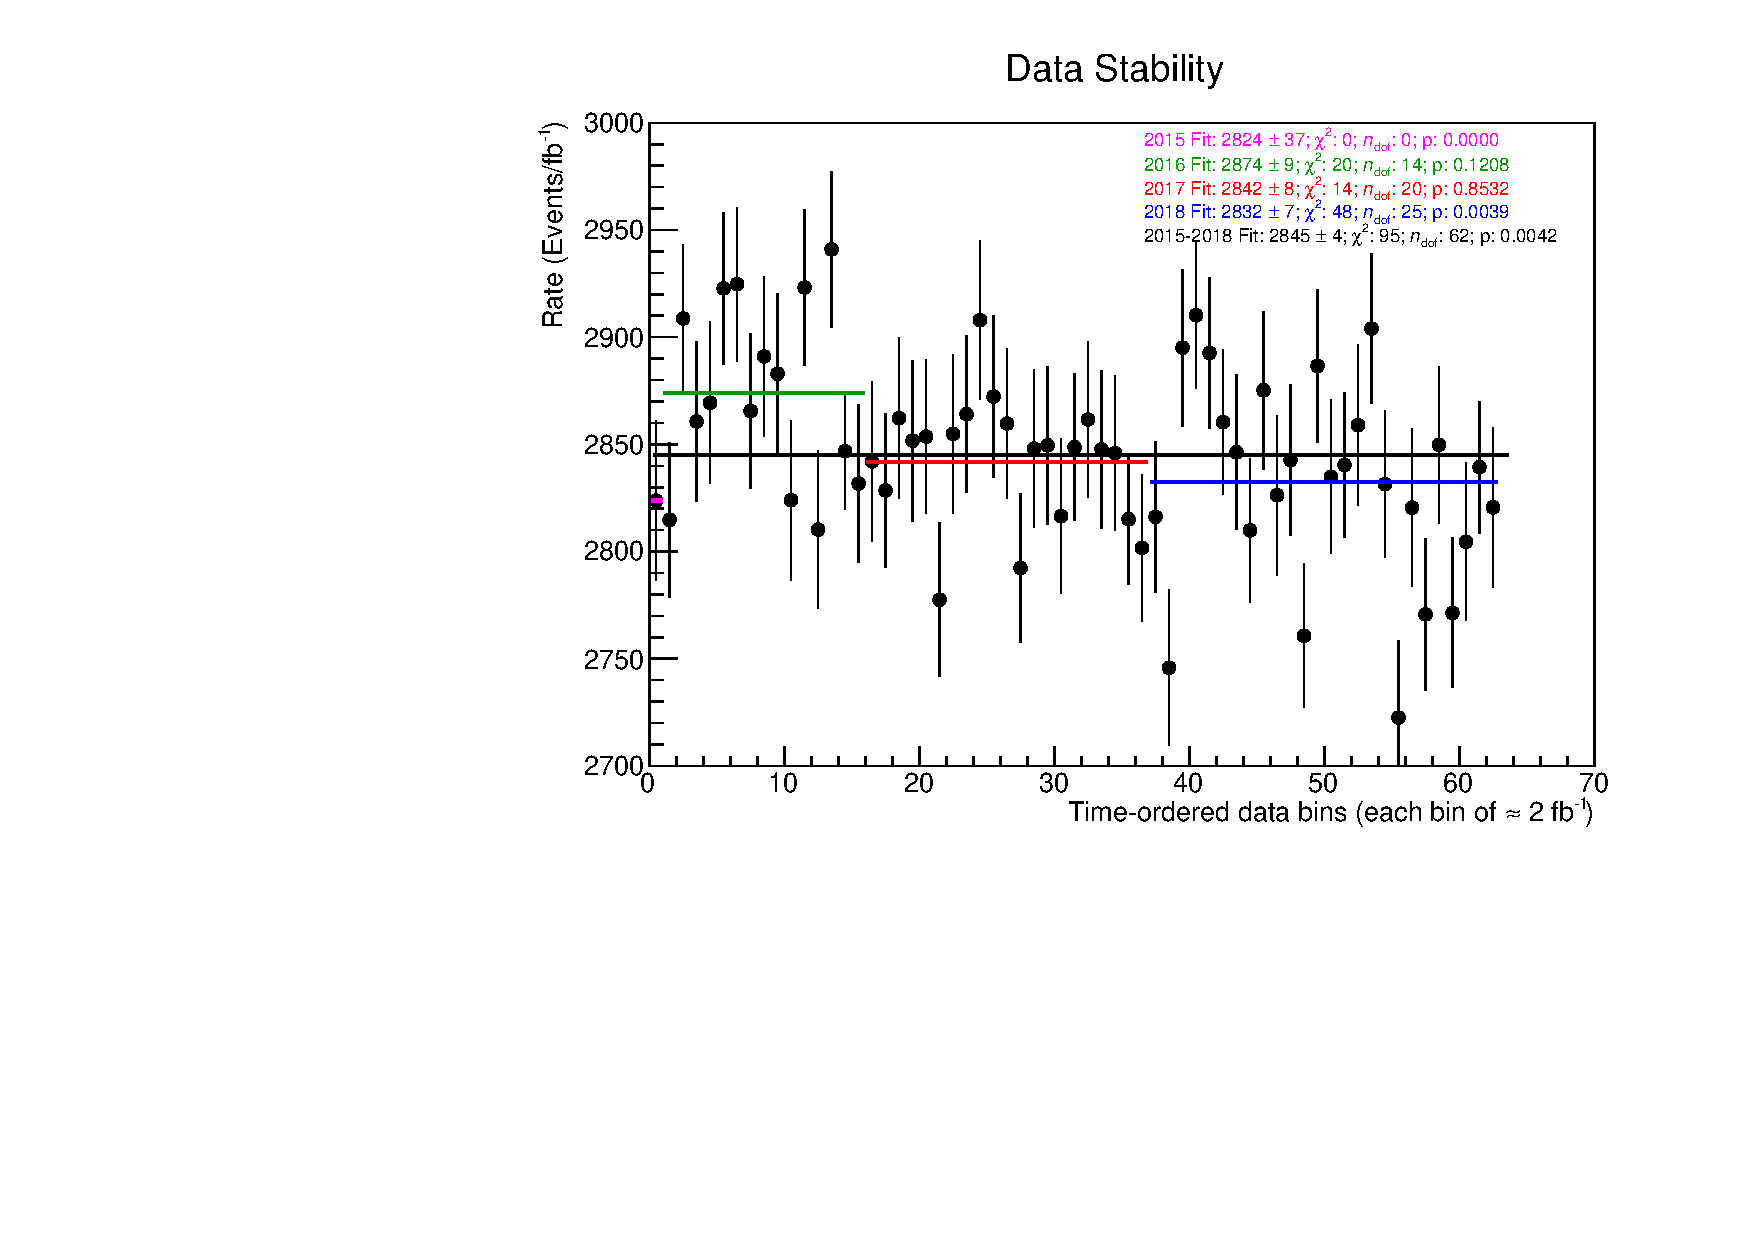
\includegraphics[width=0.75\textwidth]{figures/DataStability.pdf}
\caption{Events per fb$^{-1}$ for year 2015 to 2018, where each time-ordered data bin contains 2 fb$^{-1}$ luminosity.}
\label{fig:DataStability}
\end{figure}

\subsection{Data and Monte Carlo comparison}

Table~\ref{tab:CFComp} compares the event yields after applying the analysis cuts with data and the 2 MC samples for each year, and table~\ref{tab:RelCF} shows a relative comparison between the cuts.

\begin{table}[h!]
    \centering
    \begin{tabular}{l|l|l|l|l|l|l}
    \hline\hline
    \textbf{Sample} & \multicolumn{6}{c}{\textbf{Cuts}} \\ \hline
     & None & DQ & Trigger & Dilepton & $p_{\text{T},\ell\ell}$ & $p_{\text{T},\ell\ell}$ \\
     &  &  &  &  & $>165~\GeV$ & $>200~\GeV$ \\ \hline\hline
    Data 2015-2016 & 475.7M & 462.5M & 72.89M & 20.27M & 103.5k & 54.92k \\ \hline
    Powheg Pythia 8 MC16a & 70.63M & 70.28M & 41.27M & 20.11M & 79.31k & 41.15k \\ \hline
    Sherpa 2.2.1 MC16a & 75.60M & 75.21M & 42.28M & 20.06M & 96.72k & 52.03k \\ \hline\hline
    Data 2017 & 282.8M & 270.5M & 84.38M & 24.15M & 124.2k & 65.87k \\ \hline
    Powheg Pythia 8 MC16d & 86.42M & 85.88M & 50.35M & 24.45M & 96.58k & 50.08k \\ \hline
    Sherpa 2.2.1 MC16d & 92.50M & 91.90M & 51.59M & 24.41M & 118.3k & 63.30k \\ \hline\hline
    Data 2018 & 357.0M & 348.7M & 116.8M & 35.99M & 163.4k & 86.35k \\ \hline
    Powheg Pythia 8 MC16e & 114.0M & 113.3M & 67.22M & 32.46M & 128.2k & 66.56k \\ \hline
    Sherpa 2.2.1 MC16e & 122.0M & 121.3M & 68.93M & 36.41M & 155.9k & 83.23k \\ \hline\hline
    \end{tabular}
    \caption{Number of events remaining after each cut applied during the analysis. Data Quality (DQ) includes the GRL and event cleaning criteria.
    Dilepton includes the checks for 2 oppositely charged muons which pass TTVA and trigger matching requirements, as well as the $m_{\ell\ell}$ cut.}
    \label{tab:CFComp}
\end{table}

\begin{table}[h!]
  \centering
  \begin{tabular}{l|l|l|l|l|l}
  \hline\hline
  \textbf{Sample} & \multicolumn{5}{c}{\textbf{Cuts}} \\ \hline
    & DQ & Trigger & Dilepton & $p_{\text{T},\ell\ell}$ & $p_{\text{T},\ell\ell}$ \\
    &  &  &  & $>165~\GeV$ & $>200~\GeV$ \\ \hline\hline
   Data 2015-2016 & -2.46\% & -84.24\% & -72.20\% & -99.49\% & -46.93\% \\ \hline
   Powheg Pythia 8 MC16a & -0.50\% & -41.27\% & -51.27\% & -99.61\% & -48.11\% \\ \hline
   Sherpa 2.2.1 MC16a & -0.50\% & -43.78\% & -52.56\% & -99.52\% & -46.21\% \\ \hline\hline
   Data 2017 & -4.35\% & -68.61\% & -71.38\% & -99.49\% & -46.93\% \\ \hline
   Powheg Pythia 8 MC16d & -0.63\% & -41.37\% & 51.45\% & -99.60\% & -48.15\% \\ \hline
   Sherpa 2.2.1 MC16d & -0.64\% & -43.87\% & -52.68\% & -99.52\% & -46.51\% \\ \hline\hline
   Data 2018 & -2.30\% & -66.50\% & -72.88\% & -99.48\% & -47.04\% \\ \hline
   Powheg Pythia 8 MC16e & -0.60\% & -40.69\% & -51.70\% & -99.61\% & -48.97\% \\ \hline
   Sherpa 2.2.1 MC16e & -0.60\% & -43.17\% & -52.95\% & -99.52\% & -46.63\% \\ \hline\hline
   \end{tabular}
   \caption{The relative number of events rejected after each cut compared to the previous cut}
   \label{tab:RelCF}
\end{table}

Figure~\ref{fig:MuActual} shows the actual interactions per bunch crossing $\mu$ for the individual data periods, as well as the full Run 2 dataset.
Figure~\ref{fig:pTmll} gives the $\pt$ and $m$ distributions for the dilepton system, and figure~\ref{fig:pTetamus} gives the $\pt$ and $\eta$ distributions for both the leading and sub-leading muon.
The $\pt$ and $y$ distributions for the leading and sub-leading track jet are shown in figure~\ref{fig:pTyjets}.

Finally, the properties of the tracks used for the analysis are shown in figure~\ref{fig:trackInfo}.

\begin{figure}[h!]
  \centering
  \includegraphics[page=5,width=0.45\textwidth]{figures/ZjetOmnifoldMCDataComp.pdf}
  \includegraphics[page=6,width=0.45\textwidth]{figures/ZjetOmnifoldMCDataComp.pdf} \\
  \includegraphics[page=7,width=0.45\textwidth]{figures/ZjetOmnifoldMCDataComp.pdf}
  \includegraphics[page=8,width=0.45\textwidth]{figures/ZjetOmnifoldMCDataComp.pdf}
  \caption{The actual interactions per bunch crossing, $\mu$, for 2015-2016 data (top left), 2017 data (top right), 2018 data (bottom left), and the full Run-2 dataset (bottom right)}
  \label{fig:MuActual}
\end{figure}

\begin{figure}[h!]
  \centering
  \includegraphics[page=12,width=0.45\textwidth]{figures/ZjetOmnifoldMCDataComp.pdf}
  \includegraphics[page=16,width=0.45\textwidth]{figures/ZjetOmnifoldMCDataComp.pdf}
  \caption{Distributions for the $\pt$ and $m$ of the dilepton system. Due to the high $\pt$ phase space, it is expected that the MC simulation will underpredict the data.}
  \label{fig:pTmll}
\end{figure}

\begin{figure}[h!]
  \centering
  \subfloat[Leading muon]{\includegraphics[page=24,width=0.45\textwidth]{figures/ZjetOmnifoldMCDataComp.pdf}\includegraphics[page=32,width=0.45\textwidth]{figures/ZjetOmnifoldMCDataComp.pdf}} \\
  \subfloat[Sub-leading muon]{\includegraphics[page=28,width=0.45\textwidth]{figures/ZjetOmnifoldMCDataComp.pdf}\includegraphics[page=36,width=0.45\textwidth]{figures/ZjetOmnifoldMCDataComp.pdf}}
  \caption{The $\pt$ and $\eta$ distributions for the (a) leading and (b) the sub-leading muon}
  \label{fig:pTetamus}
\end{figure}

\begin{figure}[h!]
  \centering
  \subfloat[Leading track jet]{\includegraphics[page=72,width=0.45\textwidth]{figures/ZjetOmnifoldMCDataComp.pdf}\includegraphics[page=76,width=0.45\textwidth]{figures/ZjetOmnifoldMCDataComp.pdf}} \\
  \subfloat[Sub-leading track jet]{\includegraphics[page=88,width=0.45\textwidth]{figures/ZjetOmnifoldMCDataComp.pdf}\includegraphics[page=92,width=0.45\textwidth]{figures/ZjetOmnifoldMCDataComp.pdf}}
  \caption{The $\pt$ and $y$ distributions for the (a) leading and (b) the sub-leading jet}
  \label{fig:pTyjets}
\end{figure}

\begin{figure}[h!]
  \centering
  \includegraphics[page=128,width=0.45\textwidth]{figures/ZjetOmnifoldMCDataComp.pdf}
  \includegraphics[page=144,width=0.45\textwidth]{figures/ZjetOmnifoldMCDataComp.pdf} \\
  \includegraphics[page=148,width=0.45\textwidth]{figures/ZjetOmnifoldMCDataComp.pdf}
  \includegraphics[page=152,width=0.45\textwidth]{figures/ZjetOmnifoldMCDataComp.pdf}
  \caption{Distributions for the number of tracks per event (top left), and the $\pt$ (top right), $\eta$ (bottom left), and $\phi$ (bottom right) for each reconstructed track}
  \label{fig:trackInfo}
\end{figure}

\begin{figure}[h!]
  \centering
  \includegraphics[page=84,width=0.45\textwidth]{figures/ZjetOmnifoldMCDataComp.pdf}
  \includegraphics[page=100,width=0.45\textwidth]{figures/ZjetOmnifoldMCDataComp.pdf} \\
  \includegraphics[page=104,width=0.45\textwidth]{figures/ZjetOmnifoldMCDataComp.pdf}
    \includegraphics[page=116,width=0.45\textwidth]{figures/ZjetOmnifoldMCDataComp.pdf}\\
  \includegraphics[page=108,width=0.45\textwidth]{figures/ZjetOmnifoldMCDataComp.pdf}
      \includegraphics[page=120,width=0.45\textwidth]{figures/ZjetOmnifoldMCDataComp.pdf}\\
  \includegraphics[page=112,width=0.45\textwidth]{figures/ZjetOmnifoldMCDataComp.pdf}
      \includegraphics[page=124,width=0.45\textwidth]{figures/ZjetOmnifoldMCDataComp.pdf}
  \caption{Jet substructure features for the leading (left) and subleading (right) track jets.}
  \label{fig:jetsubstructure}
\end{figure}

\begin{figure}[h!]
  \centering
  \includegraphics[page=136,width=0.45\textwidth]{figures/ZjetOmnifoldMCDataComp.pdf}
  \includegraphics[page=140,width=0.45\textwidth]{figures/ZjetOmnifoldMCDataComp.pdf} \\
  \caption{The number of constituents in the leading (left) and subleading (right) track jets.}
  \label{fig:ntrackinjets}
\end{figure}

\clearpage


%-------------------------------------------------------------------------------
\section{Methodology}
\label{sec:strategy}

\subsection{Event selection}
Initial event selection is outlined in Table~\ref{lab:eventsel}. This is primarily designed to remove problematic and background events in favour of the $Z\rightarrow\mu\mu + \text{jets}$ signal process. The various cuts are discussed in more detail below.

\begin{table}[h!]
    \centering
    \begin{tabular}{l|l}
         \hline
    \textbf{Event Selection} & \textbf{Description} \\ \hline
    Good Runs List & Event must be part of GRL \\ \hline
    Event Cleaning & No LAr, tile calorimeter, or tracker errors. Event is complete. \\ \hline
    Trigger & Single muon trigger: \\
    & HLT\_mu20\_iloose\_L1MU15\_OR\_HLT\_mu50 (2015) \\
    & HLT\_mu26\_ivarmedium\_OR\_HLT\_mu50 (2016-18) \\ \hline
    Primary Vertex & $N_{PV}\geq1$ \\ \hline
    Muons & $N_{\text{muons}}\geq2$ \\
          & Opposite charges \\
          & Pass TTVA recommendations for muons \\
          & $81\leq m_{\ell\ell} (\text{GeV})\leq 101$ \\
          & $p_{\text{T},\ell\ell}\geq200$ GeV \\ \hline
    \end{tabular}
    \caption{Overview of the applied event selection.}
    \label{lab:eventsel}
\end{table}

\subsubsection{Event Requirements}
The first requirement is that the event must be a part of the ATLAS Good Run Lists (GRL) [GRL Ref]. These are discussed in Sec.~\ref{sec:samples}.

Secondly, the events must pass event cleaning [Event Cleaning Ref]. This removes events that:
\begin{itemize}
    \item Contain errors in the data collected in the LAr calorimeters (check for error on xAOD::EventInfo::LAr)
    \item Contain errors in the data collected in the tile calorimeters (check for error on xAOD::EventInfo::Tile)
    \item Contain errors in the silicon tracker data (check for error on xAOD::EventInfo::SCT)
    \item Events which are incomplete due to a restart of the trigger, timing and control system (check for event flag in xAOD::EventInfo::Core)
\end{itemize}

Additionally, it is required that the event in question have at least one primary vertex.

\subsubsection{Trigger Requirements}
Events are required to pass an unprescaled single muon trigger, as outlined in Table~\ref{lab:eventsel} [Trigger Ref]. The recommended trigger is dependent on the year of the data (or corresponding Monte Carlo sample).

\subsubsection{Di-Muon System Requirements}
The event is required to have at least two muons of opposite charge, with a dilepton mass between 81 GeV and 101 GeV in order to ensure the muons originate from a $Z$ boson.

Additionally, the muons must pass track-to-vertex association recommendations [TTVA ref] as follows:

\begin{itemize}
    \item $|d_0^{BL}\text{significance}| < $ 3
    \item $|\Delta z_0^{BL}\sin\theta| < 0.5 $mm
\end{itemize}

where $d_0$ and $z_0$ represent the point along the track that is the closest approach to the beamspot.

The large $p_{\text{T},\ell\ell}$ cut of 200 GeV has been chosen to ensure that the balancing jet(s) have a high quantity of charged particles, as these are the primary subject of the analysis.

\subsection{Corrections to Monte Carlo Samples}

\subsection{Data Stability Tests}

\subsection{Data and Monte Carlo Comparison}


\subsection{Unfolding Procedures}

\subsubsection{Introduction}

Paragraph introducing unfolding generally.

One of the most widely used unfolding methods is the Iterative Bayesian Unfolding (IBU) technique.  By treating each bin of a histogram as an element in a vector or matrix, we can write

\begin{align}
\textbf{R}\cdot\textbf{t}=\textbf{d}\,,
\end{align}
where $\textbf{t}$ is the particle-level distribution (represented as a vector), $\textbf{d}$ is the detector-level distribution (also represented as a vector), and $\textbf{R}$ is the response matrix.

\subsubsection{OmniFold}

\subsubsection{Illustration of Different Methods}

In order to illustrate the OmniFold procedure and how it compares to other techniques, it is useful to consider a simple two-bin example.  Suppose that there are only two possible values at particle-level and detector-level: $(T_1,T_2)$ and $(R_1,R_2)$, respectively.  Further suppose that the detector response is given by:

\begin{align}
\Pr(R_1|T_1)&=100\%\,,\\
\Pr(R_1|T_2)&=50\%\,.
\end{align}

The simulation has $\Pr_\text{MC}(T_i)=50\%$ so that $\Pr_\text{MC}(R_1)=75\%$ and $\Pr_\text{MC}(R_2)=25\%$.   Finally, we observe $\Pr_\text{Data}(R_1)=50\%$ in data.  What do the various method predict for $\Pr_\text{unfolded}(T_1)$?   Before proceeding, note that the correct answer is $\Pr_\text{Data}(T_1)=0$.

\paragraph{OmniFold}  The first step of OmniFold is to derive weights $\omega_1$ to make the MC match the data.  The weight function is specified by two numbers, one for each of the two bin values.  These weights are given by $\omega_1(R_i)=\Pr_\text{Data}(R_i)/\Pr_\text{MC}(R_i)$, which is $\omega_1(R_1)=2/3$ and $\omega_1(R_2)=2$.  These weights are then pulled back to particle level.  In MC, 50\% of events have $(T_1,R_1)$, 25\% of events have $(T_2,R_1)$ and 25\% of events have $(T_2,R_2)$.   The first two of these types of events get assigned $\omega(R_1)$ and the last one gets assigned $\omega(R_2)$.  Therefore, the weighted particle-level probability mass function is $\Pr_\text{MC,1}(T_1)=1/3$.  The second step of OmniFold derives weights $\nu_1=\Pr_\text{MC,1}(T_i)/\Pr_\text{MC}(T_i)$, which are $\nu_1(T_1)=2/3$ and $\nu_1(T_2)=4/3$. 

The above procedure is then repeated using the weights $\nu_1$ pushed to detector-level.  The new detector-level probability mass is given by $\Pr_\text{MC,2}(R_1)=2/3$.  Detector-level weights are derived according to $\omega_2(R_i)=\Pr_\text{Data}(R_i)/\Pr_\text{MC,2}(R_i)$.  Table~\ref{lab:omnifoldexample} shows the evolution of OmniFold over many iterations.

\begin{table}[h!]
\centering
\begin{tabular}{|ccccccc| }
\hline
$i$ & $\omega_i(R_1)$ & $\omega_i(R_2)$ & $\nu_i(R_1)$ & $\nu_i(R_2)$ & $\Pr_\text{MC,$i$}(R_1)$ & $\Pr_\text{MC,$i$}(T_1)$ \\
\hline
0 & 1 & 1 & 1 & 1 & $\sfrac{3}{4}$ & $\sfrac{1}{2}$ \\
1 & $\sfrac{2}{3}$ & $2$ & $\sfrac{2}{3}$ & $\sfrac{4}{3}$ & $\sfrac{2}{3}$ & $\sfrac{1}{3}$ \\
2 & $\sfrac{3}{4}$ & $\sfrac{3}{2}$ & $\sfrac{1}{2}$ & $\sfrac{3}{2}$ & $\sfrac{5}{8}$ & $\sfrac{1}{4}$ \\
\vdots & \vdots & \vdots & \vdots & \vdots & \vdots & \vdots \\
$\infty$ & 1 & 1 & 0 & 2 & \sfrac{1}{2} & 0\\
\hline
\end{tabular}
\caption{The evolution of OmniFold for the simple two-bin example described in the text.}
\label{lab:omnifoldexample}
\end{table}

\paragraph{Conditional GAN Unfolding (CGU)} In the training phase of CGU, one learns $\Pr(T_i|R_j)$ based on the simulation.  In the simple binned case, this probability mass is specified by four numbers.  

\begin{align}
\Pr(T_i|R_j)&=\frac{\Pr(R_j|T_i)\Pr(T_i)}{\Pr(R_j|T_1)\Pr(T_1)+\Pr(R_j|T_2)\Pr(T_2)}\\
&=\frac{\Pr(R_j|T_i)}{\Pr(R_j|T_1)+\Pr(R_j|T_2)}\\
&=\left\{\begin{matrix}\sfrac{2}{3} & \text{$i=1$ and $j=1$} \cr 0 & \text{$i=1$ and $j=2$}  \cr \sfrac{1}{3}& \text{$i=2$ and $j=1$}  \cr 1& \text{$i=2$ and $j=2$}  \end{matrix}\right.
\end{align}
%
Applied to data, we would measure 
%
\begin{align}
\Pr{}_\text{unfolded}(T_1)&=\Pr(T_1|R_1)\Pr{}_\text{data}(R_1)+\Pr(T_1|R_2)\Pr{}_\text{data}(R_2)=\sfrac{1}{6}\,,\\
\Pr{}_\text{unfold}(T_2)&=\Pr(T_2|R_1)\Pr{}_\text{data}(R_1)+\Pr(T_2|R_2)\Pr{}_\text{data}(R_2)=\sfrac{5}{6}\,,
\end{align}
%
which is the wrong answer.

\paragraph{Conditional Normalizing Flow Unfolding (CNFU)} In the binned case, this is equivalent to matrix inversion.   The response matrix is 

\begin{align}
\mathbf{R}=\begin{pmatrix} 1& \sfrac{1}{2}\cr 0 & \sfrac{1}{2}\end{pmatrix}\implies \mathbf{R}^{-1}=\begin{pmatrix} 1 & -1 \cr 0 & 2\end{pmatrix}\,.
\end{align}
%
Applying $\mathbf{R}^{-1}$ to $(\sfrac{1}{2},\sfrac{1}{2}$) results in $(0,1)$, the correct answer.  There are many undesirable features of matrix inversion, but it does result in an unbiased measurement.

\paragraph{Iterative Bayesian Unfolding (IBU)} 

Table~\ref{lab:ibuexample} shows the evolution of IBU over many iterations.  Note that the second column of Table~\ref{lab:ibuexample} is the same as the last column of Table~\ref{lab:omnifoldexample} - this is because OmniFold and IBU are equivalent in the binned case.

\begin{table}[h!]
\centering
\begin{tabular}{|cccccc| }
\hline
$i$ & $\Pr_\text{MC,$i$}(T_1)$ & $\Pr_0(T_1|M_1)$ & $\Pr_0(T_1|M_2)$ & $\Pr_0(T_2|M_1)$ & $\Pr_0(T_2|M_2)$\\
\hline
$0$ & $\sfrac{1}{2}$ & $\sfrac{2}{3}$ & 0 & $\sfrac{1}{3}$ & $1$\\
$1$ & $\sfrac{1}{3}$ & $\sfrac{1}{2}$ & 0 & $\sfrac{1}{2}$ & $1$\\
$2$ & $\sfrac{1}{4}$ & $\sfrac{2}{5}$ & 0 & $\sfrac{3}{5}$ & $1$\\
\vdots & \vdots & \vdots & \vdots & \vdots & \vdots  \\
$\infty$ & 0 & 0 & 0 & 1 & 1\\
\hline
\end{tabular}
\caption{The evolution of IBU for the simple two-bin example described in the text.}
\label{lab:ibuexample}
\end{table}

\subsection{Comparison of binned and unbinned}

\section{Systematic Uncertainties}
\label{sec:uncerts}


%-------------------------------------------------------------------------------
\section{Results}
\label{sec:result}
%-------------------------------------------------------------------------------


%-------------------------------------------------------------------------------
\section{Conclusion}
\label{sec:conclusion}
%-------------------------------------------------------------------------------

Place your conclusion here.


%-------------------------------------------------------------------------------
% If you use biblatex and either biber or bibtex to process the bibliography
% just say \printbibliography here
\printbibliography
% If you want to use the traditional BibTeX you need to use the syntax below.
%\bibliographystyle{bib/bst/atlasBibStyleWithTitle}
%\bibliography{ANA-STDM-2020-17-INT1,bib/ATLAS,bib/CMS,bib/ConfNotes,bib/PubNotes}
%-------------------------------------------------------------------------------

%-------------------------------------------------------------------------------
% Print the list of contributors to the analysis
% The argument gives the fraction of the text width used for the names
%-------------------------------------------------------------------------------
\clearpage
%The supporting notes for the analysis should also contain a list of contributors.
%This information should usually be included in \texttt{mydocument-metadata.tex}.
%The list should be printed either here or before the Table of Contents.
%\PrintAtlasContribute{0.30}


%-------------------------------------------------------------------------------
\clearpage
\appendix
\part*{Appendices}
\addcontentsline{toc}{part}{Appendices}
%-------------------------------------------------------------------------------
\section{Particle composition and detector response of hadronic recoil}

This section examines the particle composition and the detector response of the leading jet that balance the $Z$~boson in the fiducial region of the analysis.
The Powheg $Z\to \mu\mu$ sample is used. The particle origin of each track is obtained using the \texttt{truthParticleLink} to find the truth identification of each reconstructed track (see section~\ref{sec:samples}). In addition to the standard event preselection described in section~\ref{sec:selection}, extra cuts are used to make sure the leading reconstructed jet matches the leading particle jet in each event.
%To ensure the closet matching between the leading reconstructed jet and leading truth jet, and always have very good DR between them, the cut on ratio of
This is achieved by requiring $|y_\mathrm{j1}|<2.1$ and $\pTlj / \pTsj < 0.7$. The selection is applied on reconstructed level. However, due to the additional criterion, the leading particle-level (truth) jet will always match the leading reco jet. Note that the jets will have a very high \pt{} since the event selection includes the selection $\pTll > \SI{165}{\GeV}$, and the jet will have a similar \pt{} to that of the $Z$~boson. 

Further events are required to pass track-to-vertex association (TTVA) recommendations as described in section~\ref{subsubsec:trigger}. There are three recommending working points for \texttt{TTVA}, however studies have been done for two only i.e \texttt{loose} and \texttt{tight TTVA} selection.  

Particles are classified depending to their type in the following categories: \texttt{pion} for $\pi^+$ and $\pi^-$; \texttt{kaon} for charged kaons; \texttt{proton};
\texttt{mu} for $\mu^-$ or $\mu^+$; \texttt{e} for $e^-$ or $e^+$;
strange for any charge hadron with strange content other than kaons; \texttt{neutral} for any neutral hadron; \texttt{gam} for photons. As mentioned above, tracks are classified in the same categories using the \texttt{truthParticleLink}. In case there is no truth particle match, it is labelled unmatched. This includes contributions from pileup particles and fake tracks (and possibly secondaries).

All of the reconstructed tracks inside leading jet as well as charged-particles in the associated particle-level jets that are not matched to reconstructed tracks are used for the plots shown in this section. 

Figures~\ref{fig:r_pion_kaon} to ~\ref{fig:r_trackjet} are showing the detector response for each particle category for tight and loose TTVA working point. The pion and kaon response for \texttt{loose} and \texttt{tight TTVA} is ~94\% and ~93\% respectively.

Figure~\ref{fig:frac_unmatchedtracks} depicts fraction of unmatched track w.r.t reco level jet, which indicates ~3\% and ~8\% unmatched tracks for \texttt{tight} and \texttt{loose TTVA} working point respectively. Since \texttt{tight TTVA}  selection reduces ~5\% unmatched tracks as compare to \texttt{loose TTVA}, therefore for the current analysis we are using \texttt{tight TTVA} working point. 

\begin{figure}[b]
\centering
\includegraphics[scale=0.3, page=4]{figures/jet_comp_study_powheg_Tight_pTFraction_mc16e.pdf}
\includegraphics[scale=0.3, page=5]{figures/jet_comp_study_powheg_Tight_pTFraction_mc16e.pdf}
\caption {The response of pions (left) and  kaons (right) as a function of jet \pT. We can see that \texttt{tight TTVA} has $\approx 42$\% tracking efficiency while \texttt{loose TTVA} improved it by $\approx 1$\%}
\label{fig:r_pion_kaon}
\end{figure}

\begin{figure}[b]
\centering
\includegraphics[scale=0.3, page=6]{figures/jet_comp_study_powheg_Tight_pTFraction_mc16e.pdf}
\includegraphics[scale=0.3, page=7]{figures/jet_comp_study_powheg_Tight_pTFraction_mc16e.pdf}
\caption {The response of protons (left) and muons (right) as a function of jet \pT.}
\label{fig:r_proton_muon}
\end{figure}

\begin{figure}[b]
\centering
\includegraphics[scale=0.3, page=8]{figures/jet_comp_study_powheg_Tight_pTFraction_mc16e.pdf}
\includegraphics[scale=0.3, page=9]{figures/jet_comp_study_powheg_Tight_pTFraction_mc16e.pdf}
\caption {The response of electrons (left) and strange particles (right) as a function of jet \pT.}
\label{fig:r_electron_starnge}
\end{figure}

\begin{figure}[b]
\centering
\includegraphics[scale=0.3, page=16]{figures/jet_comp_study_powheg_Tight_pTFraction_mc16e.pdf}
\caption {The fraction of unmatched tracks w.r.t reco level jet as a function of jet \pT. We can see that \texttt{loose TTVA} has $\approx 8$\% unmatched tracks, while \texttt{tight TTVA} reduced unmatched tracks by $\approx 5$\%.}
\label{fig:frac_unmatchedtracks}
\end{figure}

\begin{figure}[b]
\centering
\includegraphics[scale=0.3, page=17]{figures/jet_comp_study_powheg_Tight_pTFraction_mc16e.pdf}
\caption {The response of  all the reconstructed tracks w.r.t charged particles as a function of jet \pT. The \texttt{loose TTVA} shows $\approx 4$\% higher track jet response than \texttt{tight TTVA}. However \texttt{loose TTVA} introduces $\approx 5$\% more tracking inefficiencies as compare to \texttt{tight TTVA} as shown in Figure~\ref{fig:frac_unmatchedtracks}.}
\label{fig:r_trackjet}
\end{figure}

For the following composition plots \texttt{tight TTVA} selection is used to study jet composition for different particles and the comparison of individual particles fraction is shown at \texttt{reco} and \texttt{truth} level.

Figure~\ref{fig:truthJetComp} shows the jet composition as a fraction of the particle multiplicity (left) and their momentum (right) as a function of the leading truth jet \pT{}. The $\approx 50$\% of reconstructed tracks make up pions about of the total, kaons are about $\approx 8$\% of the total and the rest $\approx 42$\% are neutral particles. The momentum fraction as a function of jet pT is shown in right in Figure~\ref{fig:truthJetComp}. The momentum fraction for different particles varies slightly as compare to multiplicity fraction.

\begin{figure}[b]
\centering
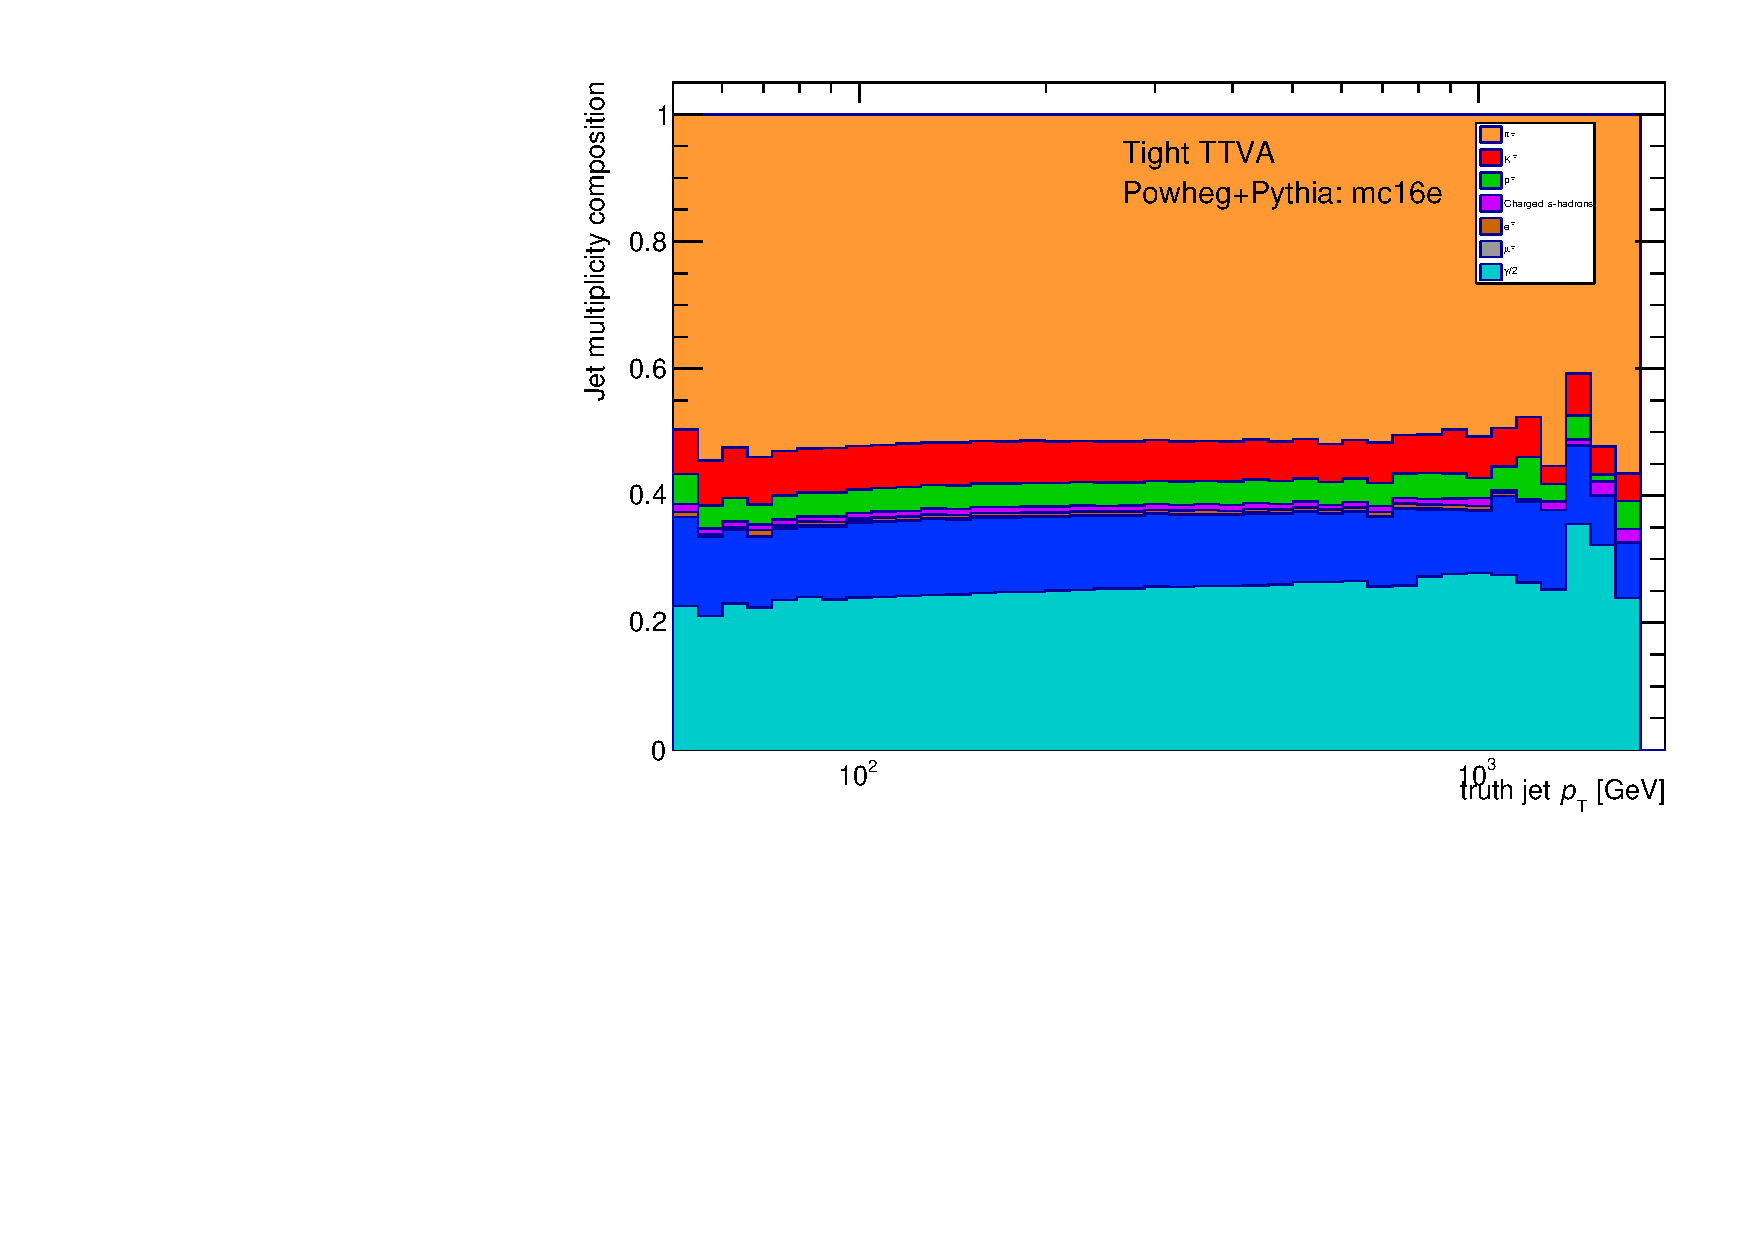
\includegraphics[width=0.48\textwidth,page=1]{figures/jet_comp_study_fixedGamma.pdf}
\includegraphics[width=0.48\textwidth,page=2]{figures/jet_comp_study_fixedGamma.pdf}%
\caption{Composition of the leading jet in terms of particle multiplicity (left) and \pt{} (right) as a function of jet \pt{}. The photon multiplicity is divided by 2 in the left plot, since most photons are produced in pairs by a neutral hadron (e.g.\ $\pi\to\gamma\gamma$).
We can see that $\approx 42$\% of the jet \pt{} is carried by neutral particles.}
\label{fig:truthJetComp}
\end{figure}

Figure~\ref{fig:chargedparticles} shows the fraction of the particle multiplicity (left) and their \pT{} as a function of the truth jet \pT in the particle-level jet. 

\begin{figure}[b]
\centering
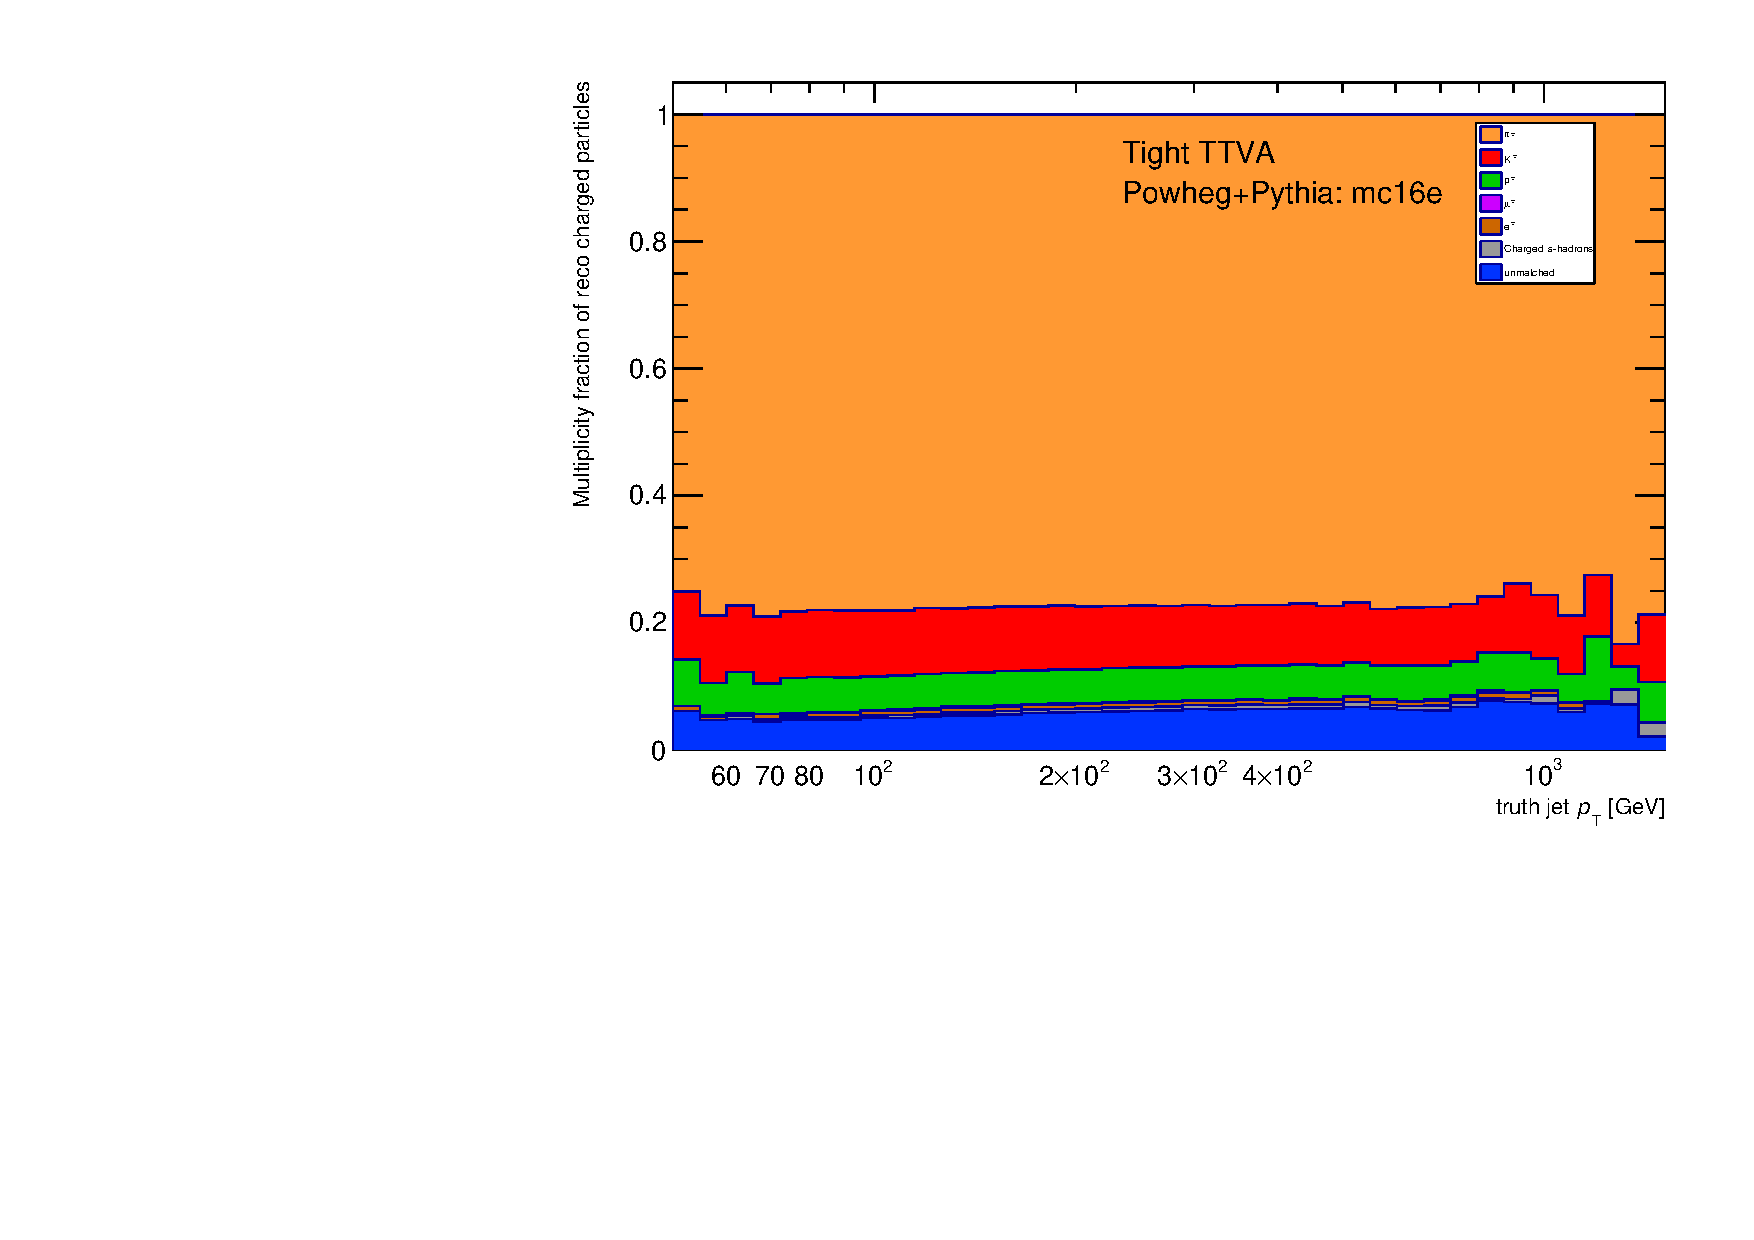
\includegraphics[width=0.48\textwidth,page=1]{figures/jetcompstudy_MultiplicityFraction.pdf}
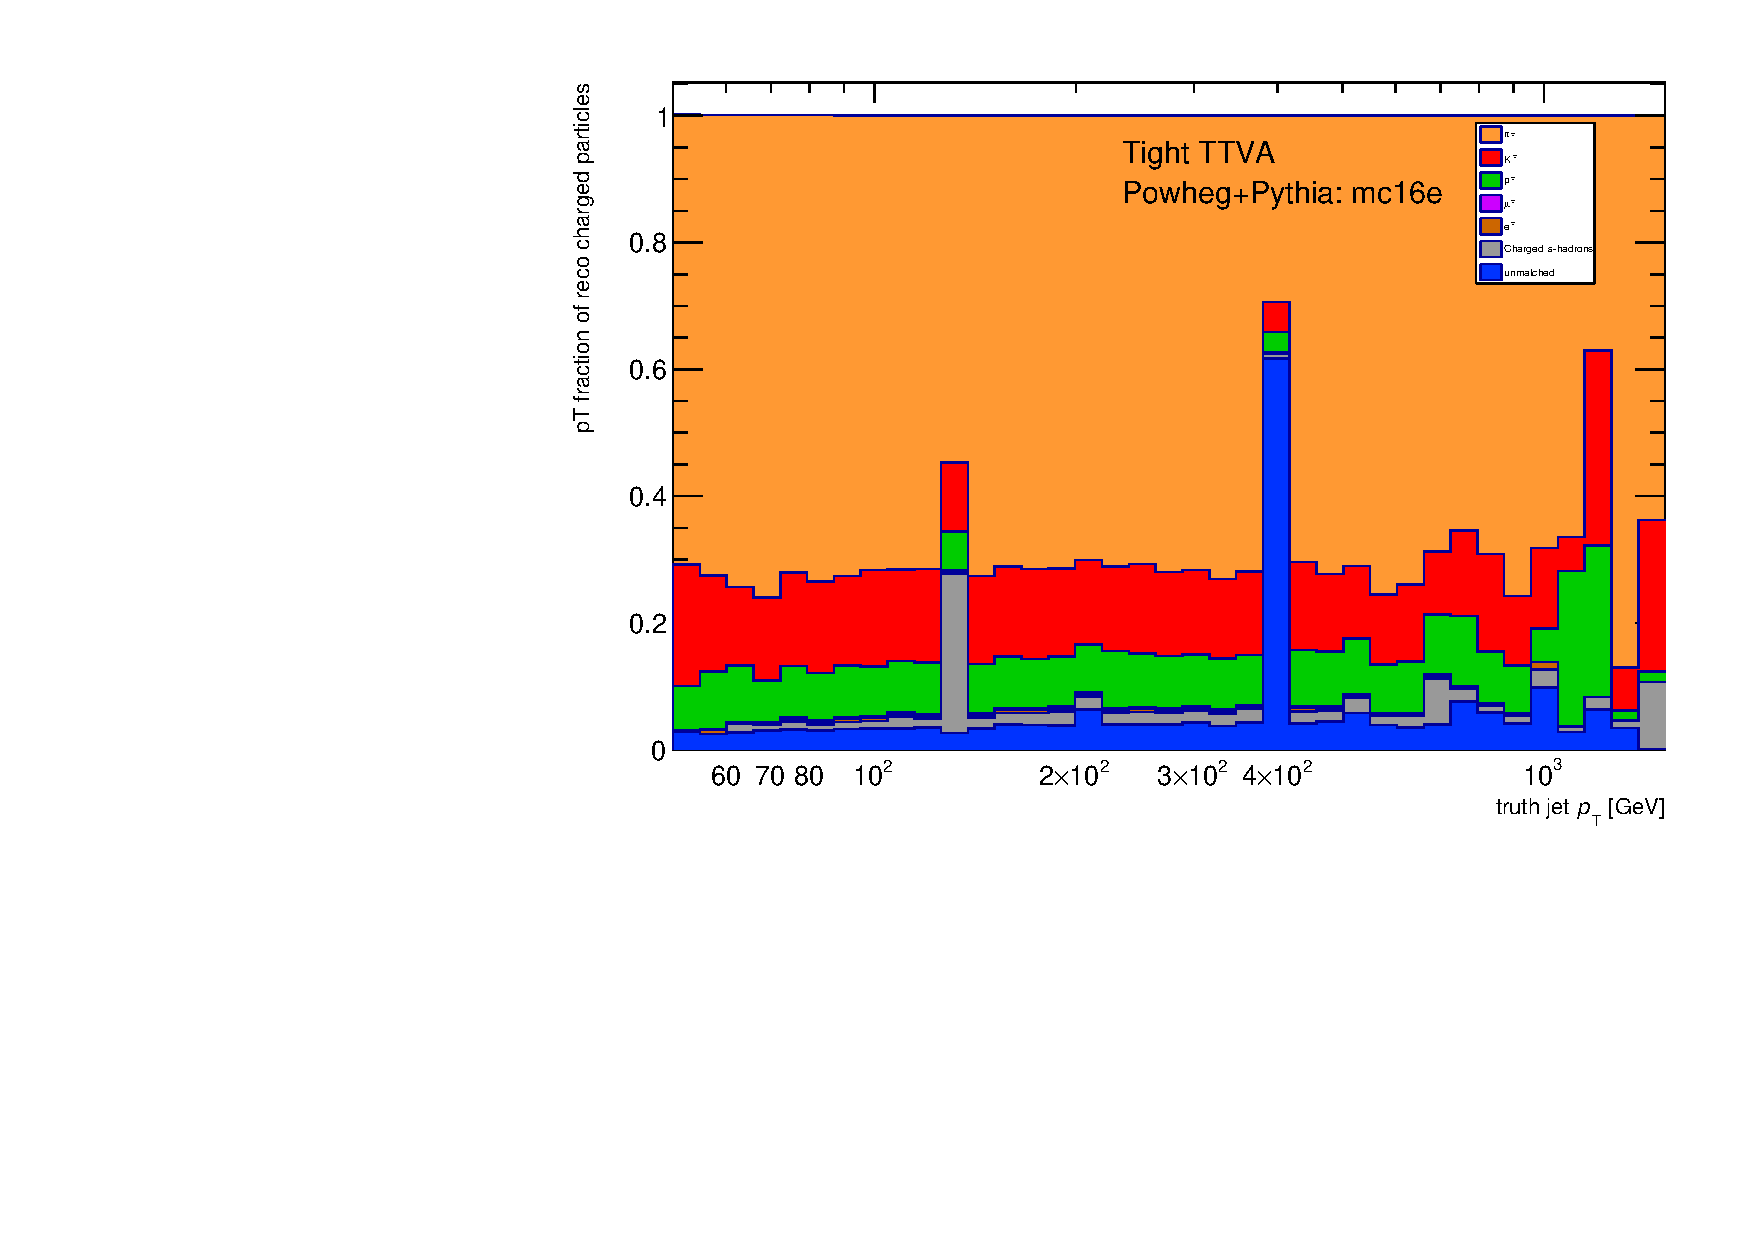
\includegraphics[width=0.48\textwidth,page=1]{figures/jet_comp_study_powheg_Tight_pTFraction_mc16e.pdf}%
\caption {The fraction of the reconstructed tracks multiplicity (left) and \pT (right) inside reconstructed leading jet as a function of jet pT for various categories. From charged particle compositions, mostly are pions $\approx71$\%, kaons are $\approx13$\% and rest $\approx16$\% comprise other charged particle.}
\label{fig:chargedparticles}
\end{figure}

Figure~\ref{fig:chargedparticles_truthjet} shows similar plots for all the charged particles compositions in the leading jet. 

\begin{figure}[b]
\centering
\includegraphics[scale=0.38, page=2]{figures/jetcompstudy_MultiplicityFraction.pdf}
\includegraphics[scale=0.38, page=2]{figures/jet_comp_study_powheg_Tight_pTFraction_mc16e.pdf}%
\caption {The fraction of the charged particle multiplicity (left) and \pT (right) inside particle level leading jet as a function of jet pT for various categories (see the text for details).}
\label{fig:chargedparticles_truthjet}
\end{figure}

Similarly, figures~\ref{fig:pions_kaons} to ~\ref{fig:electrons_sparticles} are showing the fraction of individual particles at truth level and reconstructed level. As shown in figure~\ref{fig:chargedparticles_truthjet}, pions make most of jet fraction, and for muons, electrons and strange particles this fraction is much lower. The muon and electron response is very low because these particles come from semi-leptonic decay of heavy hadrons, so we have a displaced vertex.

\begin{figure}[b]
\centering
\includegraphics[scale=0.3, page=10]{figures/jet_comp_study_powheg_Tight_pTFraction_mc16e.pdf}
\includegraphics[scale=0.3, page=11]{figures/jet_comp_study_powheg_Tight_pTFraction_mc16e.pdf}
\caption {The fraction of pions (left) and kaons (right) in the reconstructed tracks as a function of jet \pT, which shows  $\approx73$\% pions and $\approx14$\% kaons as reco level.}
\label{fig:pions_kaons}
\end{figure}

\begin{figure}[b]
\centering
\includegraphics[scale=0.3, page=12]{figures/jet_comp_study_powheg_Tight_pTFraction_mc16e.pdf}
\includegraphics[scale=0.3, page=13]{figures/jet_comp_study_powheg_Tight_pTFraction_mc16e.pdf}
\caption {The fraction of protons (left) and muons (right) in the reconstructed tracks as a function of jet \pT, which shows  $\approx7$\% proton at reco level and fraction of muons is very low.}
\label{fig:protons_muons}
\end{figure}

\begin{figure}[b]
\centering
\includegraphics[scale=0.3, page=14]{figures/jet_comp_study_powheg_Tight_pTFraction_mc16e.pdf}
\includegraphics[scale=0.3, page=15]{figures/jet_comp_study_powheg_Tight_pTFraction_mc16e.pdf}
\caption {The fraction of electrons (left) and strange particles (right) in the reconstructed tracks as a function of jet \pT.}
\label{fig:electrons_sparticles}
\end{figure}

\clearpage

\section{Monte Carlo samples}

\end{document}
